\subsection{Beschreibung der Komponenten}
Dieser Abschnitt beschreibt die physikalischen Komponenten, die von der Teilgruppe Materialfluss verwendet wurden. Zu den diesen Komponenten zählen die Rampen, sowie die \textsc{Mica}z-Module mit ihren Mikrocontrollern. 
\subsubsection{Rampen}
Rampen stellen Ein- und Ausgänge, sowie Zwischenlager im physischen System dar. Auf einer Rampe finden bis zu vier Pakete Platz. Bolzen hinter dem ersten Paket, separiert dieses von den anderen Dreien. Damit das vorderste Paket nicht vorne von der Rampe herunterfällt, sind an der Vorderseite zwei weitere Bolzen angebracht. Alle vier Bolzen sind seitlich der Rampe befestigt. Eine autonome Steuerung der Rampen, wird durch ein angebrachtes \textsc{Mica}z-Modul ermöglicht. Durch vier Lichtschranken, wird eine Überwachung der Rampe ermöglicht. Diese beinhaltet zum einen das Abfragen, wie viele Pakete auf einer Rampe liegen. Zum anderen kann durch die Überwachung überprüft werden, an welcher Stelle Pakete liegen. \autoref{fig:skiram} zeigt ein Beispiel solch einer Rampe.

\begin{figure}[h!]
	\centering
		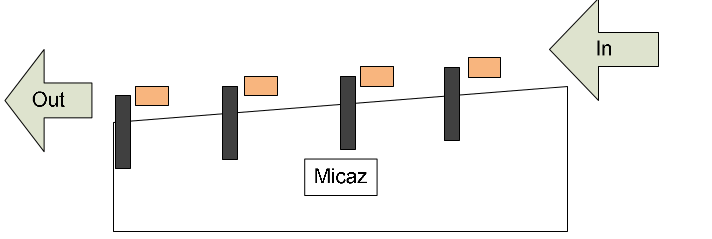
\includegraphics[width=0.9\textwidth]{SkizzeRampe.png}
	\caption{Beispiel einer eingesetzten Rampe}
	\label{fig:skiram}
\end{figure}

\subsubsection{Mikrocontroller}
Durch einen Mikrocontroller (MC) wird im Prinzip ein Mikrocomputer auf einem Chip dargestellt. Solch ein Mikrocomputer ist ein Rechner, dessen Zentraleinheit aus einem oder mehreren Mikroprozessen besteht. Zusätzlich enthält ein Mikrocomputer Speicher, ein Verbindungssystem und Ein- bzw. Ausgabeschnittstellen. Das Ziel eines Mikrocontroller ist es, eine Kommunikations- oder Steuerungsaufgabe mit möglichst wenig Bauteilen zu lösen. Der in einem Mikrocontroller verbaute Prozessorkern, Speicher und die Aus- und Eingabeschnittstellen eines Mikrocontroller, sind auf die Lösung solcher Aufgaben zugeschnitten. Die große Anzahl an potenzieller Aufgabenstellung hat zur Folge, dass es eine Vielfalt von Mikrocontrollern gibt. Meist sind die Mikrocontroller deshalb in Mikrocontrollerfamilien aufgeteilt. Innerhalb einer Familie unterscheiden sich die Controller nicht im Prozessorkern, sondern im Speicher und in den Ein- und Ausgabeschnittstellen \cite{ECHT2005}. In \autoref{fig:aufbmc} ist der schematische Aufbau eines MCs dargestellt.
\begin{figure}[th]
	\centering
		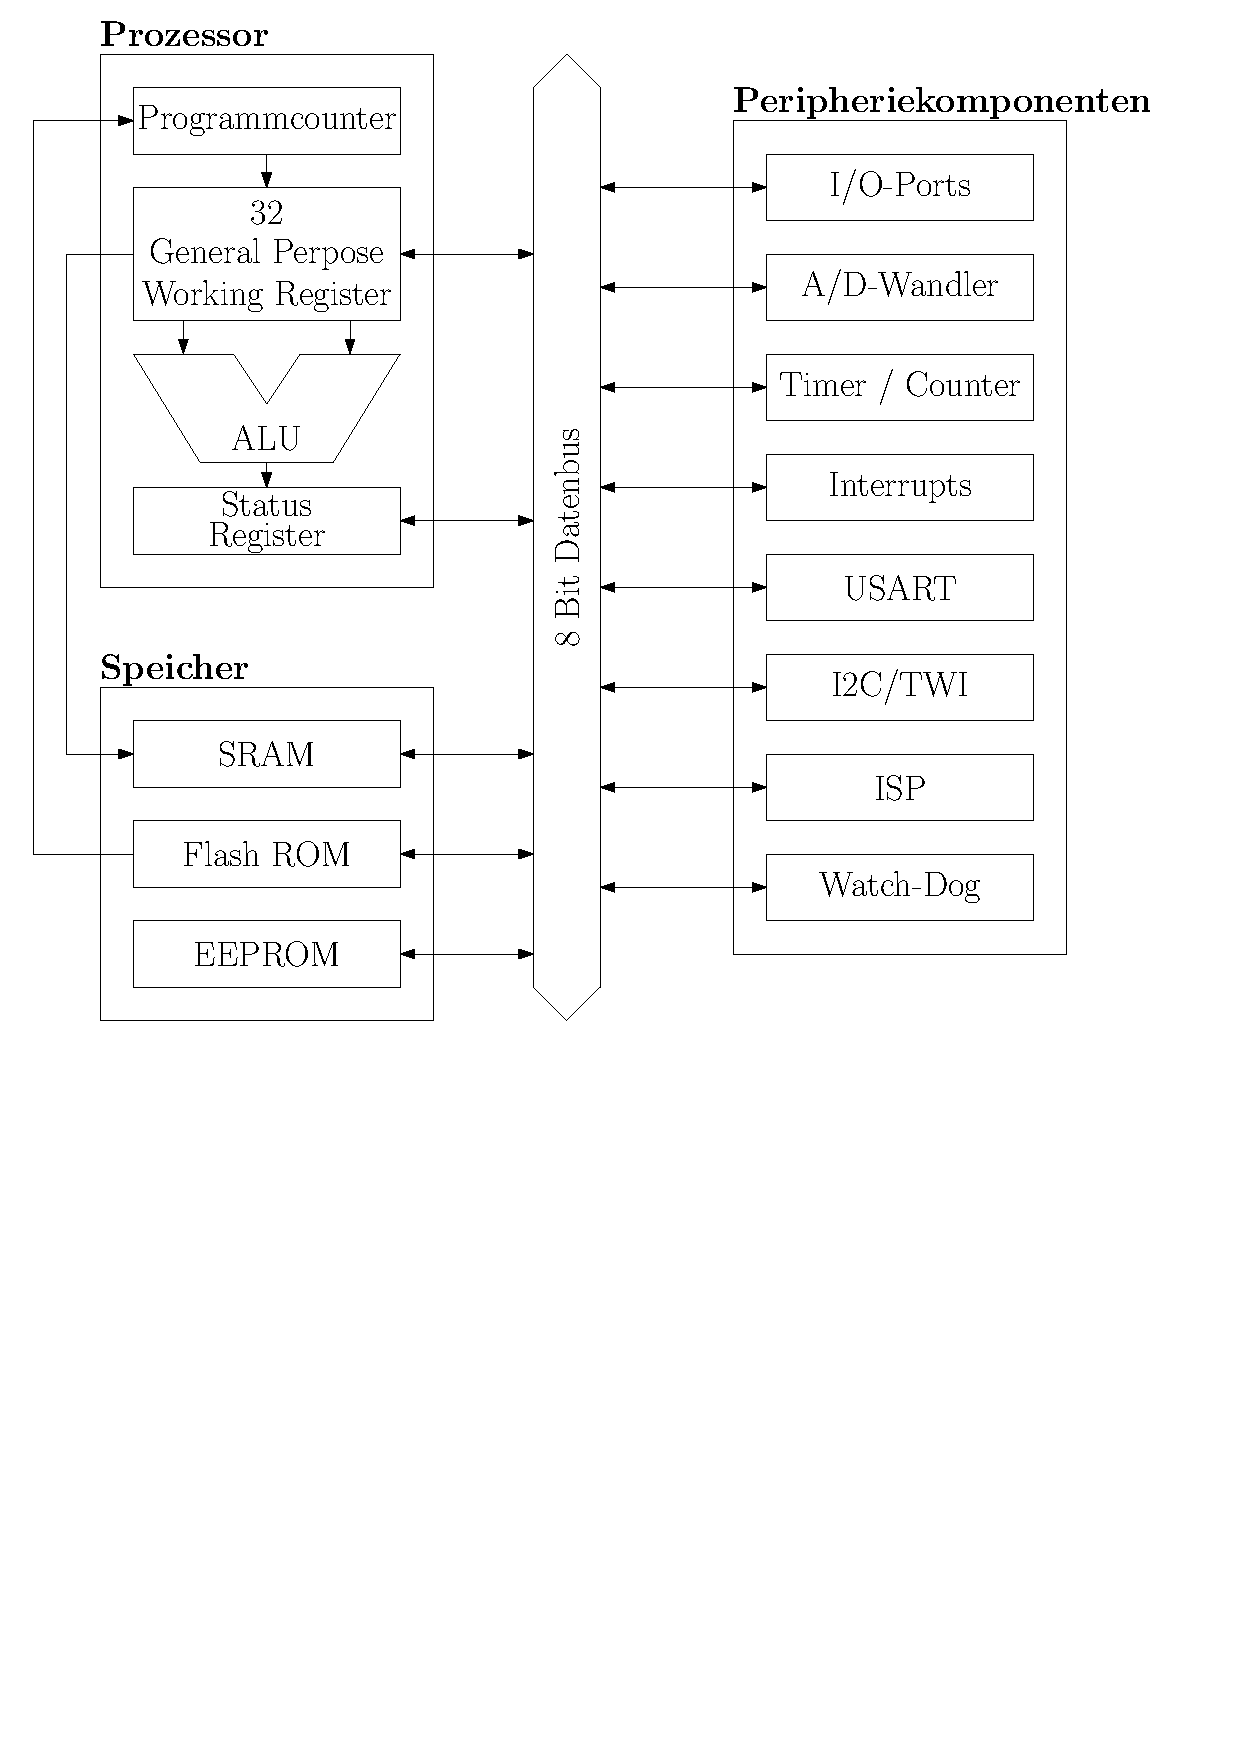
\includegraphics[width=0.8\textwidth]{flow/schemamc.pdf}
	\caption{Schematischer Aufbau eines Mikrocontrollers \cite[vgl.]{habil:Ostermeye:2014:Online}}
	\label{fig:aufbmc}
\end{figure}

Die zentrale Steuereinheit eines MCs stellt der \textbf{Prozessor} (engl.: Central Processing Unit (CPU)) dar. Sie ist die wichtigste Funktionseinheit und für die Verarbeitung von Befehlen und arithmetischen Berechnungen verantwortlich. Über den internen Bus kann die CPU mit den weiteren Grundbausteien kommunizieren und beispielsweise auf Daten innerhalb des Speichers zugreifen.

Der \textbf{Speicher} besteht in der Regel aus dem Arbeits- oder RAM (engl.: Random Access Memory) und dem Programmspeicher bzw. Flash-Speicher. Normalerweise werden diese zwei Speichertypen logisch voneinander getrennt. Programme werden im nichtflüchtigen Flash-Speicher gesichert. Dieser kann mehrere Kilobyte (KB) bis Megabyte (MB) umfassen. Bei speziellen Systemen ist es möglich den Programmspeicher durch exter-
ne Flash-Komponenten zu erweitern um zusätzlichen Speicherplatz zu ermöglichen.

Zwischenergebnisse, Messwerte von Sensoren, Steuergrößen usw. werden auf dem RAM abgelegt. Dieser ist deutlich schneller als der Flash-Speicher, hat aber in der Regel einen viel kleineren Speicherplatz. Alle Werte welche innerhalb der Laufzeit im RAM abgelegt werden, sind im Gegensatz zum Flash-Speicher flüchtig. Das bedeutet, dass nach einem Neustart des Mikrocontrollers keine Werte im RAM abgespeichert sind.

Durch die \textbf{Peripheriekomponenten} wird die Verbindung und Kommunikation zwischen Controller und Außenwelt ermöglicht. Über die digitalen Ein- und Ausgänge (I/O für Input/Output) können Sensoren und Aktoren mit dem Mikrocontroller verbunden werden. Die meisten Mikrocontroller bieten eine Vielzahl von Ein- und Ausgängen \cite[S. 13-16]{SOM2012}.

Bei der Umsetzung des Projekts wurden \textsc{Mica}z-Module eingesetzt. Im folgendem sollen diese kurz erläutert werden.sind mit einem Microcontroller aus der Atmel-Serie bestückt.

\paragraph{\textsc{Mica}z-Modul}
In \autoref{fig:blockmicaz} stellt ein Blockdiagramm der \textsc{Mica}z-Module dar. Es ist zu erkennen, dass die Module über einen ATMega128L-Mikrocontroller verfügen. Es handelt sich bei dem Controller um einen Low-Power-Mikrocontroller von der Firma Atmel. Darüberhinaus verfügt ein \textsc{Mica}z über einen CC2420-Chip der Firma Texas Instruments. Durch den Chip, wird eine drahtlose Kommunikation bei einer Frequenz von 2.4 GHz ermöglicht. Es wird dabei der IEEE 802.15.4 Standard verwendet. Eine Antenne kann über eine MMCX-Schnittstelle mit dem Modul angeschlossen werden. Weiter verfügen die Module über einen 128 KB großen Flash-Speicher. Weiter besitzen die Module eine Erweiterungsverbindung. Im Projekt wurde diese dafür genutzt, die \textsc{Mica}z-Module über ein \textsc{Mib}520 zu programmieren \cite{MICSHEET,C2420SHEET}.

\paragraph{\textsc{Mib}520}
Ein \textsc{Mib}520 stellt eine Basisstation für \textsc{Mica}z-Module dar. Zum einen kann ein \textsc{Mica}z über solch eine Basisstation an ein Computer per USB-Schnittstelle (1) verbunden werden. Dies stellt die Schnittstelle zur Teilgruppe Drive, und somit zu den Volksbots dar. Zum anderen stellt die Basistation die Möglichkeit bereit, die Module über JTAG (2) zu programmieren. Dieses ist während der Projektarbeit sehr wichtig gewesen, da ein modifiziertes Betriebssystem verwendet wurde. Außerdem wurden über diese Methode selbstgeschriebene Treiber, Interfaces und andere auf das \textsc{Mica}z-Modul übertragen und somit erst zur Verfügung gestellt \cite{MICSHEET}.

\begin{figure}[th]
  \centering
    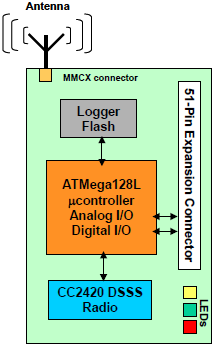
\includegraphics[width = 0.5\textwidth]{flow/blockmicaz.PNG}
    \caption{Blockdiagramm der \textsc{Mica}z-Module}
    \label{fig:blockmicaz}
\end{figure}
%\paragraph{Sensorik und Aktorik}
%Hauptziel der Teilgruppe Materialfluss ist das Management von Paketen auf einer Rampe.
%Die Aufgabe der Sensorik ist dabei, dass die mit Lichtschranken ausgestatteten Rampen Pakete detektieren und auf Änderungen der Positionen der Pakete reagieren.
%Die Lichtschranken bestehen aus einer Lichtstrahlenquelle (dem Sender) und einem Sensor (dem Empfänger) f\"{u}r diese Strahlung.
%Als Lichtquelle kommt Infrarotlicht zum Einsatz und der Vorteil besteht in der einfachen Einstellung des Sensorsystems durch den
%sichtbaren Lichtfleck. Das Funktionsprinzip der Lichtschranke besteht darin, den sich  ändernden Zustand durch die Lichtintensität mit dem Sensor zu registrieren. 
%Die Rampen werden auf Hardwareebene um eine Aktorik zum Arretieren der Kisten ergänzt. Diese Aktoren (in unserem Fall die
%eingesetzte Bolzenpaare) sind für das Ausführen von Bewegungen zuständig.
%Sie sind aktive Stellelemente, die in der Antriebs- und Steuerungstechnik vom  Mikrorechner angesteuert werden, um das Verhalten des Prozesses durch das vom Sensor kommende Signal in einer gew\"{u}nschten Weise zu ermöglichen. In dieser allgemeinen Darstellung stehen die 
%Ausgangssignale eines Sensors und die Stellsignale der Aktoren mit einem
%Informationsverarbeitungssystem (IVS) in Verbindung.
